\section{Evaluation}
\label{sec:evaluation}
How are we checking the validity of the goodness-criteria for splits? The examples below show that the algorithm captures the goodness criteria...
Data characteristics: what about cases where it splits crossing lines or the bullseye pattern?
Something about performance?

\subsection{Examples}
\subsubsection{Visual Patterns}
To illustrate the ability of our approach to pick out interesting Partitioners based on different visual patterns, we look at data about American universities and different Scagnostic measures. The Integrated Postsecondary Education Data System (IPEDS) is the primary source for data on colleges, universities, and technical and vocational postsecondary institutions in the United States via the National Center for Education Statistics.\footnote{\url{http://public.tableau.com/s/resources?qt-overview_resources=1}} We are interested in understanding the relationship between the percent of admitted students and the graduation rate of students with Bachelors degrees within $6$ years as in Figure~\ref{fig:original1}. 
\begin{figure}
 \centering 
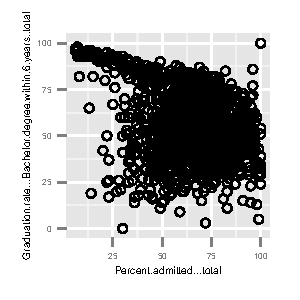
\includegraphics[width=2.25in,height=2.25in]{images/original1.pdf}
  \caption{Original interesting bivariate relationship}
 \label{fig:original1}
\end{figure}

\begin{figure}
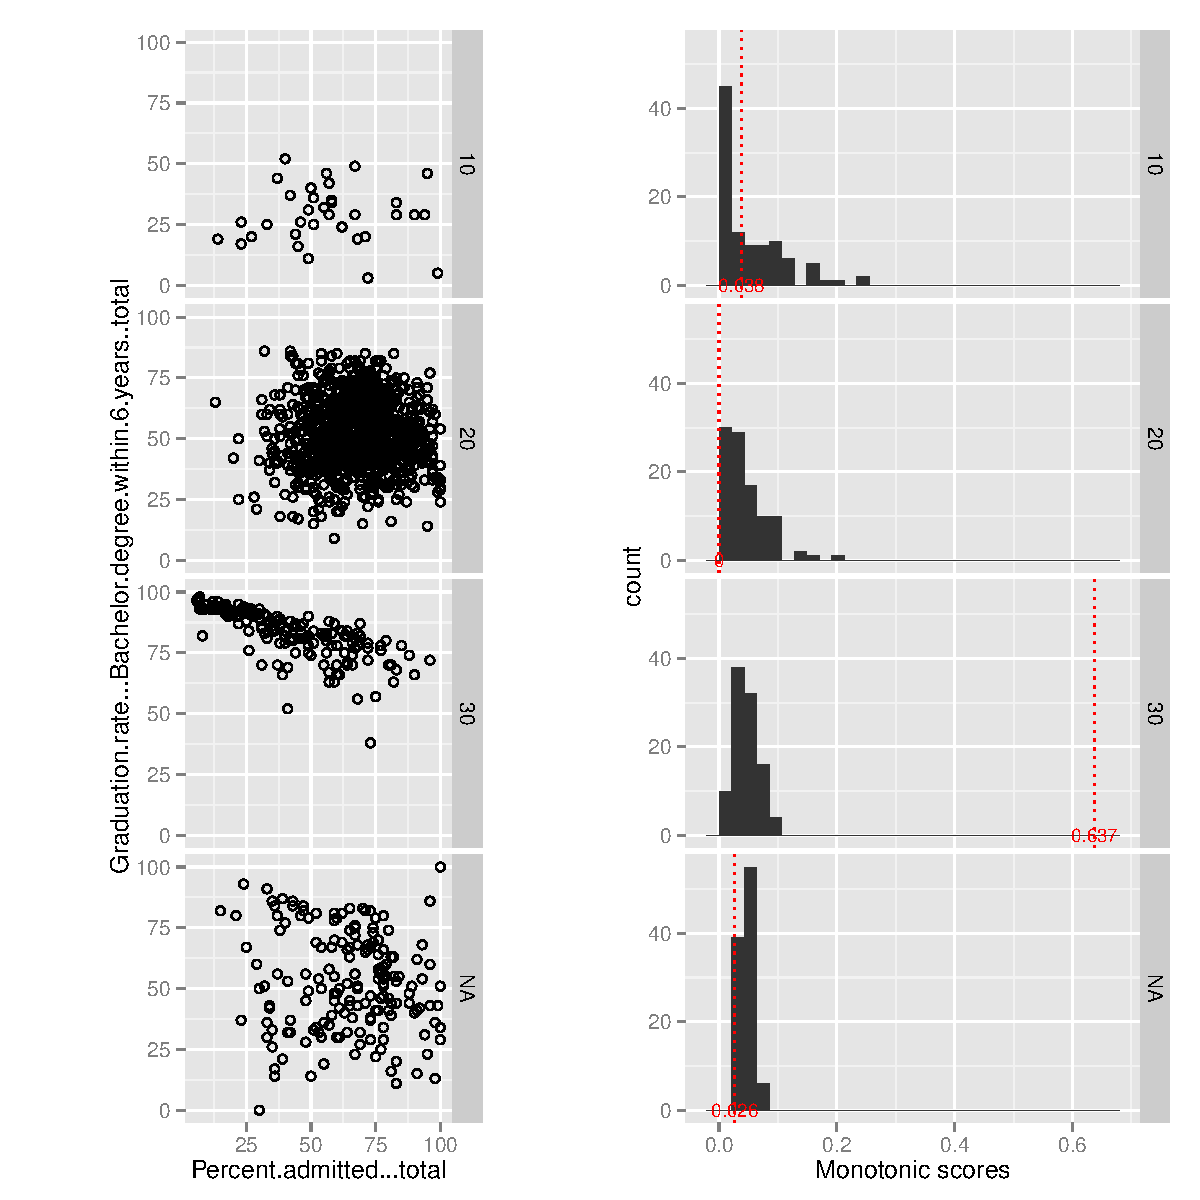
\includegraphics[width=4in,height=4in]{images/15_8918450338241-ACT_Composite_75th_percentile_score_bin.pdf}
  \caption{Monotonic}
 \label{fig:monotonic1}
\end{figure}

With the Monotonic Scagnostic as the measure to score splits, the highest ranked Partitioner is the variable labeled ACT\_Composite\_75th\_percentile\_score\_bin. This variable represents a disjoint, simple binning of the ACT Composite 75th percentile score into four categories, one of which is ``NA" - missing data code. Figure~\ref{fig:monotonic1} shows the resulting split with clearly interesting visual patterns in each facet of the resulting small multiple on the left. This Partitioner has succeeded in pulling apart revealing structure from the original bivariate relationship giving us a visual explanation of elements of the pattern in Figure~\ref{fig:original1}. 
The splits $\left\{{10, 20, 30, NA}\right\}$ have sizes $\left\{{36, 1010, 153, 335}\right\}$. Each histogram on the right shows the distribution of the Monotonic score on the bootstrapped samples of the same size as the facet it is aligned with on the left. The vertical, red, dashed line is a reference line for the score of the visual pattern in the left plot, so it can be visually compared to the reference distribution. In this case the strong Monotonic pattern in bin $30$ is a significant divergence from the expected range of values for the Monotonic score given the dataset and random samples without replacement of size $153$.

\begin{figure}
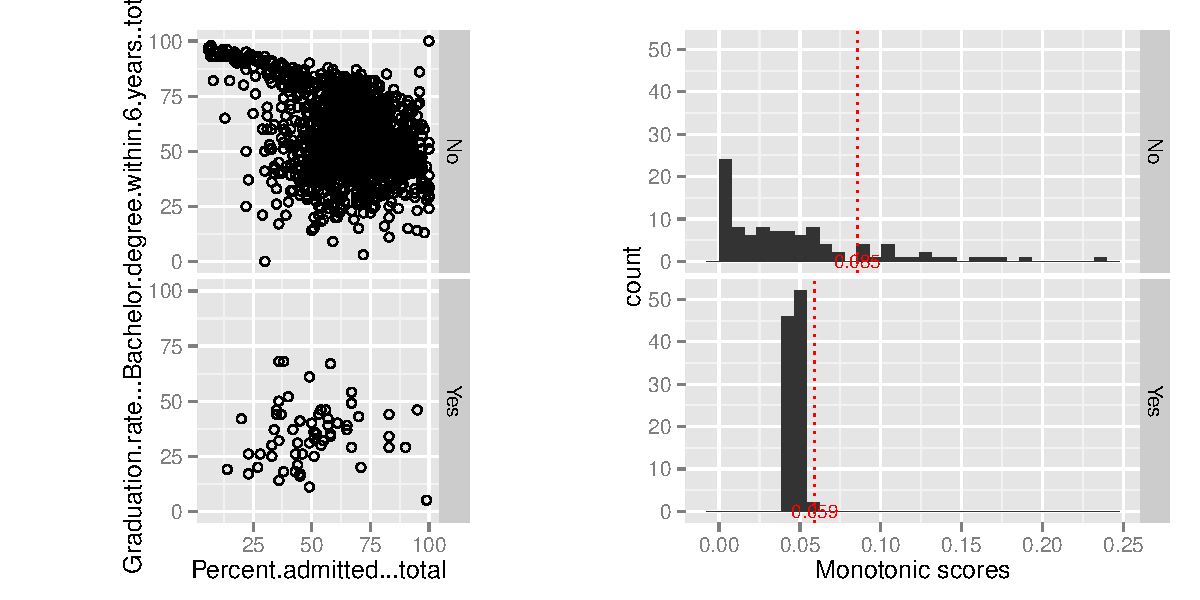
\includegraphics[width=4in,height=2.5in]{images/10_3880027387531-Historically_Black_College_or_University.pdf}
  \caption{Outlying}
 \label{fig:outlying1}
\end{figure}

Selecting a different Scagnostic measure such as Outlying, ranks a different split as the most salient as seen in Figure~\ref{fig:outlying1}. Here, the Partitioner variable Historically\_Black\_College\_or\_University produces a split that maximizes the z-score criterion over other variables despite not having a significant Outlying score on any facet as compared to the reference distributions seen on the right. The Outlying score considers the overall shape and density of the points in a two-dimensional point cloud so small relatively evenly distributed sets of points will have low scores as seen in the distribution of the $81$ points for the ``Yes" category in relation to the $1453$ points in the ``No" category.

\subsubsection{Divergence}
Different -- Can it pick out ``confounding variates" such as those that cause Simpson's Paradox?

\subsubsection{Support}
Low support cases would have low scores.
support -- small n (ourworld.csv) vs large n. small -> inside distributions so we'll be more conservation in judgements of "real" patterns.
 1 example plot. small amount. random split looks like a a pattern.. well inside distribution successful detected not real pattern.
\begin{figure}
 \centering 
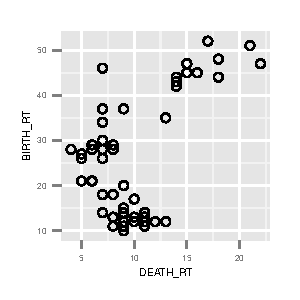
\includegraphics[width=2.25in,height=2.25in]{images/BIRTH_RT-DEATH_RT.pdf}
  \caption{Original interesting bivariate relationship}
 \label{fig:original2}
\end{figure}

\begin{figure}
\raggedleft
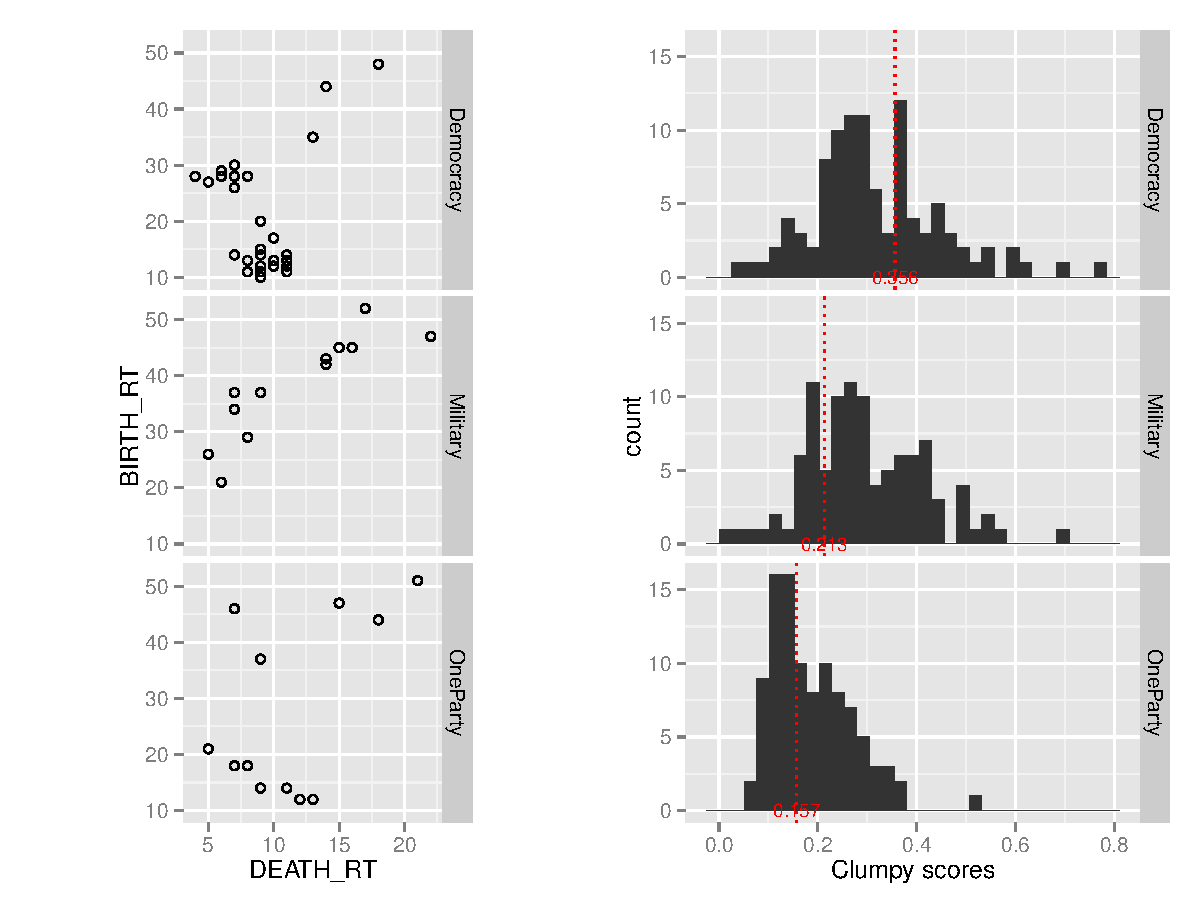
\includegraphics[width=3.75in,height=3.5in]{images/2_05954102971921-GOV.pdf}
  \caption{clumpy}
 \label{fig:clumpy1}
\end{figure}

\subsubsection{Degrees of Freedom}
High-cardinality Partitioners create a large number splits, which allow for more
 -- State vs Region

\section{Discussion}
\label{sec:discussion}
Our approach of selecting Partitioner variables that showcase interesting visual explanations is generalizable in terms of allowing for a diversity of measures used to capture ``interesting visual structure". The wide range of measures surveyed~\cite{Bertini2011} can be used w/ our method based on the plot type of interest to describe the visual pattern of interest to find when partitioning a view.

Furthermore, we can use this approach of selecting good splits of a data view to guide other multivariate exploratory data analysis applications.

Decision tree approach of guided EDA.

Trellis displays present a grid of plots of the same type showing the same variables conditioned on a Partitioner variable that determines the subsets of points shown in each plot. These displays are a very useful multivariate display as they are simple to interpret and provide an overview of large datasets for exploratory data analysis. Crucial to the layout of small multiples is the selection of a Partitioner variable to specify faceting into plots by rows and/or columns. This choice can then be repeated to facet the resulting plots further applying crossing and nesting.


